\documentclass[journal,twocolumn,10pt]{IEEEtran}
\pagestyle{plain}

\usepackage[acronym]{glossaries}
\newacronym{IEEE}{IEEE}{Transactions on Information Forensics and Security}

\usepackage{epsfig}
\usepackage{booktabs}
\usepackage{multirow}
\usepackage{blindtext}
\usepackage{xcolor}
\usepackage[ampersand]{easylist}
\usepackage[]{algorithm2e,algorithmicx}
\usepackage[bottom]{footmisc}
\usepackage{graphicx}
\usepackage[tight,footnotesize]{subfigure}
\usepackage{booktabs}
\usepackage[colorlinks, linkcolor=blue,anchorcolor=black,citecolor=blue]{hyperref}

\renewcommand{\sectionautorefname}{\S}
\renewcommand{\subsectionautorefname}{\S}
\renewcommand{\subsubsectionautorefname}{\S}

\usepackage{textcomp}
\usepackage[T1]{fontenc}
\usepackage[utf8]{inputenc}

\makeglossaries

\title{Establishing Trusted I/O Paths for \\ SGX Client Systems with Aurora}

% Author(s) Name
\author{Hongliang~Liang,~\IEEEmembership{Member,~IEEE,}
	Mingyu Li,~Yixiu Chen,~Lin Jiang,~Zhuosi Xie,~Tianqi Yang\\
	Trusted Software and Intelligent System Lab.,
	Beijing University of Posts and Telecommunications\\
	\{hliang, maxul, chenyixiu, jianglin, xiezhuosi, yangtianqi\}@bupt.edu.cn\\
%	\thanks{H. Liang, M. Li, Y. Chen, L. Jiang, Z. Xie, T. Yang are with Trusted Software and Intelligent System Lab, Beijing University of Posts and Telecommunications, Beijing 100876, China. e-mail: (\{hliang, maxul, chenyixiu, jianglin, xiezhuosi, yangtianqi\}@bupt.edu.cn) }% <-this % stops a space
    \thanks{This work was supported by the National Natural Science Foundation of China (NSFC) under Grant No. U1713212 and 91418206.}
}

\begin{document}

\maketitle

\begin{abstract}

Today users' private data in edge computing devices (desktops, laptops, and tablets, etc.) is at high risk because they run applications on potentially compromised or malicious systems. To address this problem, hardware vendors propose Trusted Execution Environment (TEE). Particularly, Intel has released a new processor feature called Software Guard eXtension (SGX), and provisions shielded executions (i.e., enclaves) for security-sensitive computations. Regrettably, Intel SGX's design objectives omit trusted I/O paths. Without such guarantees, it is unlikely for an enclave to fulfill its security and privacy purposes because the source or sink of data may have been corrupted.

To this end, we propose a novel architecture called \textsc{Aurora} to provide trusted I/O paths for enclave programs even in the presence of untrusted system software.
Specifically, \textsc{Aurora} exploits two commercial-off-the-shelf features (System Management Mode, SMM and SGX) and establishes a secure channel between an enclave program and target device.
Furthermore, we design and implement trusted paths for HID keyboard, serial port printer, hardware clocks, and USB mass storage, respectively. Leveraging these trusted paths, we protect real-world applications including OpenSSH client, OpenSSL server/client and SQLite database.
Security and performance evaluations show that \textsc{Aurora} mitigates several kinds of I/O related attacks and introduces acceptable overheads.

\end{abstract}

\begin{IEEEkeywords}

Trusted Path, Hardware Trust, Intel SGX, System Security

\end{IEEEkeywords}



\section{Introduction}

%% 从定义出发 “可信计算” 的定义出发,可信计算包含五个组件
%% 云环境下安全问题众多(引用云攻击综述);用户安全与隐私问题受人关注,IntelSGX应运而生,已有不少工作,例如针对原装二进制、数据分析、网络中间件等一系列工作横空出世,都很好地利用SGX自身的特点,那就是内存对外不可见。但是缺乏对安全IO的保证。
Trusted computing~\cite{DBLP:journals/ieeesp/Felten03} encompasses six key technologies including: 1) endorsement key, 2) protected execution, 3) sealed storage, 4) secure input and output, 5) remote attestation, and 6) trusted third party. To this end, Intel provisions Software Guard eXtensions (SGX) \cite{DBLP:conf/isca/McKeenABRSSS13} to establish trusted execution environment that protects the integrity and confidentiality of desired computation. Intel SGX enforces strong isolation in memory for security-sensitive compartments in a user-level application, called \textit{enclaves}, from untrusted privileged systems. Many SGX-based protection architectures~\cite{DBLP:journals/tocs/BaumannPH15,DBLP:conf/osdi/HuntZXPW16,DBLP:conf/osdi/ArnautovTGKMPLM16,DBLP:conf/icdcs/NguyenG17,7545819,DBLP:conf/sp/SchusterCFGPMR15} have already been proposed to secure data and code on untrusted servers.

%% 比较可惜的是,这项技术本身并没有为数据的通道做任何加固。一个只计算不交互的应用几乎是不存在的,比如上面提到的工作,都对IO的吞吐做了评测。也就是说,SGX 不保护数据的安全进出,只保护计算过程本身。对于不可靠的数据,我们认为计算是没有价值的,例如时间。这些都和SGX技术自身设计的出发点有关,那就是归根结底要依赖不可信的OS。
Unfortunately, Intel SGX enclaves have no direct access to any hardware resources because Intel SGX by design does not support any secure input/output mechanisms according to its Software Developer's Manual~\cite{Corporation2016Intel}. Concerning I/O requests, an enclave has to rely upon the untrusted compartments through system call interfaces. This unreliable dependency is susceptible to attacks such as memory-based Iago attacks~\cite{DBLP:conf/asplos/CheckowayS13} and I/O-based traffic analysis~\cite{DBLP:conf/ccs/MittalKJCB11}.

A trusted path between an enclave program and a target I/O device is a protected channel that assures the secrecy and authenticity of transferred data. It is extremely critical to user's privacy on personal computers, such as health information, financial account and personal documents, etc. The private data can be protected inside an enclave during runtime, but it is impossible to protect it at the time of being printed since typically printer devices only understand plaintext data and the corresponding drivers are under the control of the untrusted kernel. Similarly, the textual input from users such as keystrokes can be recorded on a compromised computer, which is a very serious problem when it comes to password security~\cite{DBLP:conf/uss/SilverJBCJ14}. Previous research like SafeKeeper \cite{DBLP:conf/www/KrawieckaKPMA18} only protects the password on the server side, but cannot protect the user's password from keylogging threats on the client side.

%% 以时间为例,LibOS的shield模块对系统毫无检验的能力;一些必须依赖正确时间的区块链程序只好去远程取绝对时间;Intel虽然在17 年从AMT/ME给出了可信时间服务,但依旧没有妥善解决这个问题,那就是高频时间戳请求下的精度问题。结果就是,来Intel自家的OpenSSL库都要用系统ftime接口,得到毫秒精度时间戳。
Intel SGX enclaves also suffer from the loss of a high-precision trusted clock. State-of-the-art library OSes such as Haven~\cite{DBLP:journals/tocs/BaumannPH15}, Graphene-SGX~\cite{DBLP:conf/usenix/TsaiPV17} and Panoply \cite{shinde_panoply:_2017} rely on the clock value from  untrusted systems. As a result, these systems are vulnerable to time deception attacks~\cite{DBLP:conf/ccs/ChenZRZ17}. Blockchain-oriented systems like Town Crier~\cite{DBLP:conf/ccs/ZhangCCJS16} depend on a remote server for a trusted time; however, this clock latency is high (usually hundreds of milliseconds) and uncertain. Intel Management Engine (ME) offers a trusted clock service for SGX enclaves, but the time value is coarse-grained (second-resolution) and not absolute at all \cite{intel_psw}. It is not satisfactory for those enclaves that request the timestamp information at a high frequency, (e.g., tens or hundreds of times per second). Hence, to achieve millisecond-resolution time, Intel SGX SSL~\cite{intel_sgx_ssl} has to use \textit{ftime}, offered by the OS, which contradicts original SGX threat model. Cryptographic libraries such as TaLos~\cite{TaLoS}, mbedTLS-SGX~\cite{mbedtls}, WolfSSL-SGX~\cite{wolfSSL} encounter the same problem as well. Additionally, another trusted service named Intel monotonic counters are slow and the NVRAM used by it only supports limited times of writes \cite{DBLP:conf/uss/MateticAKDSGJC17}.

%% 我们不禁要反诘:如今的方案真的能保护好Enclave吗?尤其是那些会和不可信OS 交互的enclave?如果不行,我们继续问:那么到底怎样才能做好呢?所以,本文就是要探索一种方法,给SGX程序强有力的IO安全保护,本质还是为了保护enclave。当然,我们的场景设在云上,没有变。
%As for some enclave programs that require human interactions like keyboard/mice input and display on the screen,
Today's SGX ecosystem has not yet come up with an off-the-shelf solution to trusted I/O paths. Enclaves themselves cannot authenticate whether they are communicating with trusted devices or not. It is significantly important to solve the problem on \textbf{\emph{how to establish trusted I/O paths for enclaves on untrusted systems}}, as almost all SGX-based projects exclude the underlying OS from the trusted computing base (TCB) while awkwardly depending on it for I/O requests.

%% 所以,我们有了Aurora,专门提供可信IO服务的Aurora,它负责为enclave提供一条直达IO设备的可信路径。这个方法引入了一个可以执行特权指令、访问IO 设备的特殊“enclave”,即系统管理模式RAM。它是现有X86架构下的一块高特权飞地,同一模式下的飞地外代码、其他模式都无法访问和修改它。我们在SMRAM 和enclave间构建本地的可信路径,就能很好地给enclave提供绕过不可信区域的IO可信路径!
On Intel platforms, we observe that 1) all peripheral I/O devices are connected with south-bridge to I/O Advanced Programmable Interrupt Controller (I/O APIC), 2) I/O interrupts can be rerouted to System Management Interrupt (SMI) via configuring I/O APIC and 3) the SMI handler is initialized by Unified Extensible Firmware Interface (UEFI) which contains kinds of device drivers; thus, we hold the insight that \textit{the SMI handler} is a perfect candidate to provide trusted I/O paths for security-critical applications.

In this paper, we present \textsc{Aurora}, a novel architecture that safeguards I/O paths of SGX enclaves. To directly communicate with hardware devices without depending on the untrusted software, \textsc{Aurora} introduces System Management RAM (SMRAM) as a special enclave. SMRAM is a tamper-proof memory region used only in System Management Mode (SMM), much like the enclave region with SGX protection in user mode. \textsc{Aurora} delegates I/O requests from enclaves to the SMI handler protected inside SMRAM. We call this particular SMI handler \textit{SMVisor}. In hardware, SMVisor is safe from any corruptions by other privileged software. Therefore, Intel SGX enclaves can safely use I/O devices while remaining \textit{transparent} to the underlying OS and hypervisor.

%% 我们的贡献点有:Aurora是个全新的系统服务框架;四款全新的服务;实际的应用评估证明其可用性。
To summarize, this paper makes these contributions:
\begin{enumerate}[]
\item The notion of two types of trusted I/O paths: data-provider/-consumer path and data-storage/-transmitter (\autoref{types}) path, for security-sensitive applications (enclave programs).
\item A novel architecture named \textsc{Aurora} (\autoref{arch}) leveraging two hardware features of Intel processors (SMM and SGX) to provide enclaves trusted paths transparent to untrusted OSes/HVs with a minimal trusted computing base (\autoref{codebase}).
\item Design and implementation of four types of trusted I/O paths (\autoref{tpaths}): keyboard, printer, clock, and storage, based on \textsc{Aurora}.  To the best of our knowledge, we are the first to provide these \emph{realistic} trusted I/O paths for SGX enclaves on the client side.
\item Three case studies: OpenSSH client, OpenSSL client, and SQLite database using trusted I/O paths provided by \textsc{Aurora} (\autoref{casestudy}). Experimental results show that \textsc{Aurora} can protect them from typical I/O related attacks (\autoref{security}) with acceptable performance overhead (\autoref{performance}).
\end{enumerate}

\begin{figure*}[t]
	\centering
	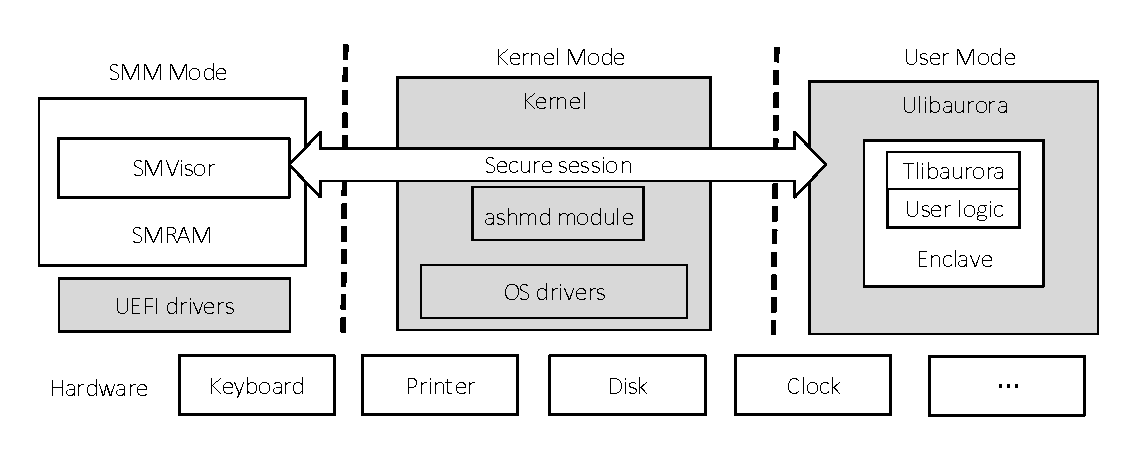
\includegraphics[height=0.22\textheight]{figures/arch.pdf}
	\caption{\textsc{Aurora}'s architecture. The gray areas denote untrusted parts, and the white ones represent \textsc{Aurora}'s trusted computing base.}
	\label{fig:architecture}
\end{figure*}

\section{Background and Problem Definition}
In this section, we first describe two architecture features of Intel's CPU, and then propose two types of trusted I/O paths based on the characteristics of devices. Finally, we describe the threat model and assumptions.

\subsection{Software Guard eXtension}
Intel SGX \cite{DBLP:conf/isca/McKeenABRSSS13} provides trusted execution environments called enclaves in user level. Enclaves' code and data reside in a hardware-protected memory named enclave page cache (EPC), which is inaccessible to any software including OS/HV or SMI handler. Enclave code can access the memory outside the enclave. As enclave code is only allowed to be executed in user mode, any interaction with devices must execute outside of the enclave and through untrusted system calls. SGX enables a threat model where users only trust the Intel CPUs and the code running inside the enclaves.

Intel SGX SDK provides a function call mechanism for enclaves via ECALL and OCALL.  Thus, an application can invoke an enclave's code via an ECALL and get the return values. The enclave can invoke an OCALL to execute a function in the untrusted portion of the application and receive a return value. SGX provisions remote attestation and local attestation \cite{Anati2013InnovativeTF}. With SGX's remote attestation ability, one can gain confidence that the target application is securely running within an enclave. Local attestation allows an enclave to prove to one another that it is running on the same processor.

\subsection{System Management Mode}
System Management Mode (SMM) \cite{Corporation2016Intel} is the most privileged mode for handling system-wide functions like power management, etc. Upon a system management interrupt (SMI), the CPU saves the system context and switches to SMM, and executes a predefined logic (SMI handler) in system management memory (SMRAM). We deem SMRAM as a special \textit{enclave}, because SMRAM cannot be accessed by OS/HV after initialization, and therefore protects the confidentiality and integrity of SMI handler. An \textit{RSM} (resume) instruction is executed to switch back to the protected mode.

The SMI handler is initialized by UEFI, and  SMRAM can be locked by configuring \emph{D\_OPEN} and \emph{D\_LCK} bits in SMRAM control register. Therefore, the SMI handler is safe from tampering after boot. Moreover, the SMI handler can access all CPU registers, I/O devices, and physical memory (except for SGX EPCs), and thus we expand the SMI Handler to design \textsc{Aurora}'s SMVisor in \autoref{arch}.

\subsection{Trusted I/O Paths}\label{types}

%% 传统的UNIX系统将设备分为字符设备、块设备和网络设备。每种设备都有自己的I/O端口号、IRQ中断号以及对应的物理内存。字符设备是最为原生的设备,这些设备包括鼠标、键盘、实时时钟、串口等。这些设备要么产生电平数据作为CPU的输入,要么得到CPU的输出作为指示。我们将此类设备归类为“生产/消费设备”。块设备和网络设备负责数据的持久化保存和在计算节点间传输,他们自身不产生也不消耗带有信息的数据,我们根据其功能将其命名为“存储/传输设备”。我们观察并认为所有的设备都可以归结为这两类,并为这两类设备与程序间构建可信路径。由于分类的不同,可信路径的工作原理也不同。参考Zhou,我们依旧将可信路径的组成分成三个组件:设备端、程序端和通信路径。“生产/消费设备”模型下可信路径要求设备的数据/指令必须通过通信路径传输。这是因为,这些设备参与了数据的产生或使用,而硬件自身并不支持加密协议来保证数据的隐私,这种情况下,我们需要在设备端引入新的TCB对数据做密码学处理。相比之下,“存储/传输设备”只是被动地接收或发送已有的数据,保护隐私的加密运算可以单独放在程序端完成。类型的不同导致了设计的不同,甚至实现代价也不同。我们会在后文中说明。
%% 面向“生产/消费设备”考虑隐私数据的保护,而面向“存储/传输设备”的可信路径用于对攻击检测、预期行为验证等。
We define \emph{trusted I/O paths} in trusted execution environments (TEEs, e.g. SGX) as follows. Given a trusted application (e.g. an SGX enclave) and a trusted peripheral device, a trusted I/O path is a secure channel of data transfers between them, even in the face of software adversaries such as host kernel, hypervisor, guest VM and kernel drivers. We classify trusted I/O paths into two categories based on their characteristics:

\begin{enumerate}

\item \textbf{Data-provider/-consumer type.}
Although SGX provides user-space strong isolation for program end-points (i.e. enclaves), most of the devices provide and/or consume plaintext messages. Cases vary from human input data (e.g., keyboard scan code) to outputted data (e.g., a stream of bits to printer/display), which cannot guarantee the confidentiality and integrity in an untrusted or compromised system. Therefore, for trusted paths of this kind, \textsc{Aurora} encrypts/decrypts in SMRAM the data from/to devices for enclaves to protect the data from the untrusted system.

\item \textbf{Data-storage/-transmitter type.} Storage disks and network adapters are typical storage/transmitter devices. Both kinds of devices can deal with encrypted data without knowing the semantics of the data. However, both devices need a pile of software stacks (e.g., file system, network protocol) to work correctly and remain compatible. Building trusted paths for them is very challenging. One possible approach is to decompose existing software stack and port them into the trusted applications, which will greatly swell the TCB and attack vectors \cite{weiser_sgxio:_2017}. As an alternative, \textsc{Aurora} leverages a \emph{verify-then-use} method that reuses existing software stacks in a secure manner (\autoref{driver}).

\end{enumerate}

The main difference between these two types is that \textit{data-provider/-consumer} is either the sink or the source of data and must handle data in plain-text, which requires careful isolation or confidential protection; Whereas the \textit{data-storage/-transmitter} type acts as a medium for data at rest or in transition. It focuses on the freshness and integrity of data.

\subsection{Threat Model and Assumptions}
We consider an adversary who can compromise the system via software attacks. He can directly attack enclave interfaces visible to the OS, and actively reconfigure any devices (e.g., modify MMIO region, or change the operating mode of a device) and perform arbitrary operations (e.g., trigger interrupts, issue DMA write requests) using any I/O commands.

\textsc{Aurora} requires a modern Intel platform with SGX and TPM support. We assume the hardware and SMRAM firmware (the microkernel we implement) of the host machine is trusted. We do not trust the UEFI drivers but verify whether they operate following their specifications, or perform unintended operations: e.g., intercept bus traffic, or write to an address that is not specified in DMA commands. Our assumptions  reduce the TCB on the target host as modern commodity system usually contains a large software stacks (e.g., UEFI, possibly hypervisor, kernel and other applications) when dealing with I/O devices.
Physical attacks on devices, side-channel attacks~\cite{chen2019sgxpectre, ridl}, information leakage (I/O size and request/response frequency) and denial-of-service attacks to Aurora's framework are not considered. The adversary cannot access the physical machine and modify its hardware setup. %we adopt side-channel free cryptographic algorithms and apply an oblivious packet transferring technique (\autoref{enhancement}).


\section{Design}
%% 我们用的是SMM和SGX两种CPU特性组成的“可靠、可信”系统服务。Aurora命名缘由。
To provide trusted I/O paths, we employ the combination of SGX and SMM, both of which are processor enforced protection features. Because they are offered at the opposite ends of Intel privilege-level model, we name our framework after \textsc{Aurora}\footnote{Aurora takes place in the polar regions, \emph{i.e.,} south and north of the earth.}.

%% SMM call,代理+模拟 模式。Enclave的请求最终在SSV处得到响应,和syscall、vmcall是一个道理。
Establishing a trusted path in \textsc{Aurora} consists of the following three steps. First, \textsc{Aurora} builds a secure session between SMVisor and an enclave that performs an I/O request. Second, SMVisor receives the request via the secure session without leaking knowledge to the untrusted system. Third, SMVisor interacts with the target device on behalf of the enclave, and performs desired I/O operations for the request. The procedure is conceptually similar to a \textit{syscall} or \textit{vmcall}. We name this an \textit{smcall} for brevity.

\subsection{Architecture}\label{arch}

\textsc{Aurora} is composed of three components: SMVisor, libaurora and a secure session established between SMVisor and libaurora, as shown in Figure \ref{fig:architecture}.

%% SMVisor 负责判断中断源/设备,调用驱动,以此提供服务。SSV对驱动模型有限制。
%% libaurora 把SGX缺少的IO相关接口补上,方便移植
%% SSV和libaurora之间有信道连接
\begin{enumerate}%[(1)]
\item SMVisor takes charge of the target devices from the untrusted kernel. It dispatches device interrupts to either kernel or enclaves. SMVisor securely invokes UEFI drivers outside of SMRAM (\autoref{driver}).
\item Libaurora consists of two parts. The trusted part (Tlibaurora) complements unsupported I/O APIs in Intel SGX SDK library, helping developers secure enclave's I/O paths. The untrusted part (Ulibaurora) is responsible for forwarding \textit{smcalls} to SMVisor.  %; an ENCLAVEID can be obtained using \textit{EREPORT} instruction
\item The secure session exchanges encrypted messages between SMVisor and an enclave via a shared memory provided by a kernel module named ashmd.  \textsc{Aurora} leverages a 5-tuple: \textit{(ENCLID, DEVID, OPTYPE, PAYLOAD, MAC)} for each message. The first two arguments indicate the program endpoint and device endpoint respectively.  The third stands for the type of I/O operation. The fourth carries the message data and the last is the message authentication code used for integrity protection. All the arguments are marshaled and encrypted. 

\end{enumerate}

\begin{figure}
	\centering
	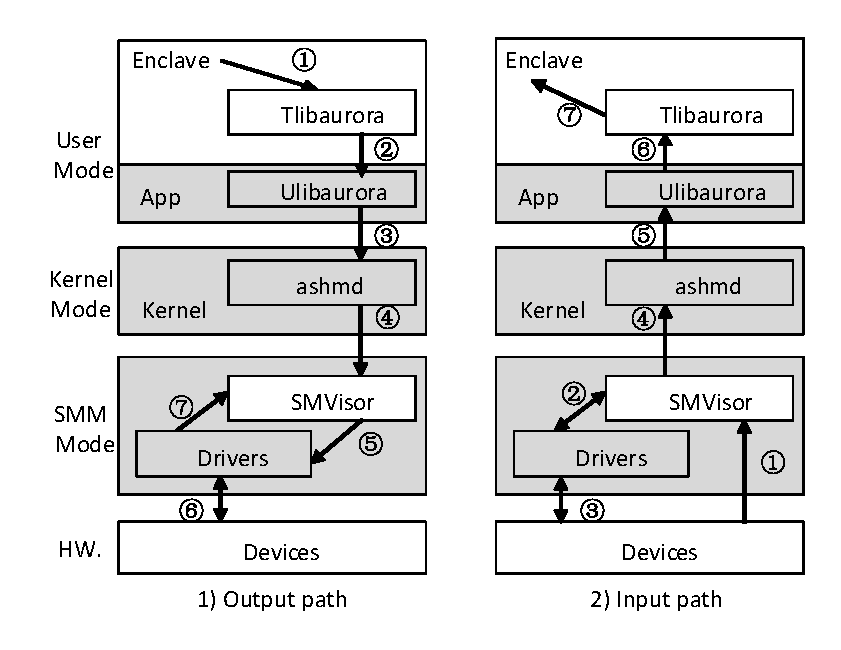
\includegraphics[width=0.49\textwidth]{figures/workflow.pdf} %height=0.25\textheight,
	\caption{The workflow of a trusted I/O path in \textsc{Aurora}. %The white areas denote the TCB.
	1) An \textbf{output} request is triggered by an enclave as an exception:
\textcircled{\scriptsize{1}} The user logic in an enclave issues an output request by invoking  Tlibaurora's APIs;
\textcircled{\scriptsize{2}} Tlibaurora marshals and encrypts the request's arguments, and invokes Ulibaurora outside the enclave to relay the request;
\textcircled{\scriptsize{3}} Ulibaurora \emph{ioctls} the ashmd module to trigger an \textit{smcall};
\textcircled{\scriptsize{4}} SMVisor is notified and obtains the encrypted requests from the secure session;
\textcircled{\scriptsize{5}} SMVisor decrypts the request and invokes the driver;
\textcircled{\scriptsize{6}} The driver processes output data in PCI space or MMIO buffer;
\textcircled{\scriptsize{7}} The driver returns a result code to SMVisor. In the end, SMVisor executes \textit{RSM} to return to protected mode. 
	2) An \textbf{input} request from an enclave causes a device interrupt:
\textcircled{\scriptsize{1}} The target device triggers an interrupt, and the control flow is rerouted to SMVisor which has the interrupt handler;
\textcircled{\scriptsize{2}} SMVisor invokes the driver to handle the input request;
\textcircled{\scriptsize{3}} The driver gets the raw input data and sends it to SMVisor;
\textcircled{\scriptsize{4}} SMVisor encrypts the data inside SMRAM, and sends it to the target enclave via the secure session;
\textcircled{\scriptsize{5}} The system switches back to protected mode and the ashmd module uses a signal to notify Ulibaurora;
\textcircled{\scriptsize{6}} Ulibaurora invokes Tlibaurora to receive the encrypted data;
\textcircled{\scriptsize{7}} The enclave decrypts the encrypted data and finally obtains the raw input data.
	}
	\label{fig:workflow}
\end{figure}

To help understand the workflow of a trusted path in \textsc{Aurora}, we break down the process of the output path and input path respectively into sequential phases, as illustrated in left and right part of \autoref{fig:workflow}.

%% 和LibOS一样,我们也是要减小对不可信OS的依赖,我们甚至没有和OS交互的数据流接口,只有中断对其是不透明的。
%% 但又和LibOS不一样,我们连驱动都不用不可信OS的,以此保证数据来源的可靠性和流出的不受干扰。
Like library OSes~\cite{DBLP:journals/tocs/BaumannPH15, DBLP:conf/usenix/TsaiPV17, shinde_panoply:_2017}, \textsc{Aurora} has few interfaces with the untrusted OS. %Only interrupts are forwarded by the OS to SMVisor.
The data plane of an enclave is protected by advanced encryption schemes accelerated by the processor (\emph{i.e.,} AES-GCM with AES-NI support), and the data flows between the enclave and SMVisor are completely invisible to the OS. Unlike library OSes, which delegate I/O operations to the untrusted OS, \textsc{Aurora} ships security-sensitive parts of these operations into SMVisor, thus eliminating the reliance on untrusted OS.

\iffalse

\subsection{Workflow}\label{workflow}

To help understand the workflow of a trusted path in \textsc{Aurora}, we break down the process of the output path and input path respectively into sequential phases, as illustrated in left and right part of \autoref{fig:workflow}.

An output request is triggered by an enclave as an exception, as depicted as follows:\\
%\par
~~\textcircled{\footnotesize{1}} The user logic in an enclave issues an output request by invoking  Tlibaurora's APIs;\\
~~\textcircled{\footnotesize{2}} Tlibaurora marshals and encrypts the request's arguments, and invokes Ulibaurora outside the enclave to relay the request;\\ %sends the request via the secure session, via an OCALL
~~\textcircled{\footnotesize{3}} Ulibaurora \emph{ioctls} the ashmd module to trigger an \textit{smcall};\\
~~\textcircled{\footnotesize{4}} SMVisor is notified and obtains the encrypted requests from the secure session;\\
~~\textcircled{\footnotesize{5}} SMVisor decrypts the request and invokes the driver;\\
~~\textcircled{\footnotesize{6}} The driver processes output data in PCI space or MMIO buffer;\\
~~\textcircled{\footnotesize{7}} The driver returns a result code to SMVisor. In the end, SMVisor executes \textit{RSM} to return to protected mode. \\

\par
An input request from an enclave causes a device interrupt, as depicted as follows:\\
%\par
~~\textcircled{\footnotesize{1}} The target device triggers an interrupt, and the control flow is rerouted to SMVisor which has the interrupt handler;\\
~~\textcircled{\footnotesize{2}} SMVisor invokes the driver to handle the input request;\\
~~\textcircled{\footnotesize{3}} The driver gets the raw input data and sends it to SMVisor;\\
~~\textcircled{\footnotesize{4}} SMVisor encrypts the data inside SMRAM, and sends it to the target enclave via the secure session;\\
~~\textcircled{\footnotesize{5}} The system switches back to protected mode and the ashmd module uses a signal to notify Ulibaurora;\\
~~\textcircled{\footnotesize{6}} Ulibaurora invokes Tlibaurora to receive the encrypted data;\\
~~\textcircled{\footnotesize{7}} The enclave decrypts the encrypted data and finally obtains the raw input data. % from the secure session.
\fi

\subsection{SMVisor}\label{ssv}

SMVisor is the core component in \textsc{Aurora}.  It may take charge of multiple devices simultaneously, therefore it needs to determine which device is being requested and then invokes the corresponding driver. 

%% 数据来的时候首先被SSV拦下,判断好了再转发,避免OS污染隐私数据
%It protects the device ends from any other logical attacks. When SMVisor receives a request, it takes control of the target device interrupts to prevent the untrusted system from interrupt spoofing attacks.
\textbf{Interrupt Handler.} To deal with a device interrupt, SMVisor reroutes the interrupt to SMI. Specifically, SMVisor intercepts device events by configuring the \textit{Redirection Table} defined in I/O APIC and modifying the destination of the device event to SMI. SMVisor distinguishes the interrupt source and thus notifies a certain enclave or the untrusted kernel. In order to forward the interrupt to upper software layer, it issues an inter-processor interrupt (IPI) by writing the interrupt command request (ICR) register in the local APIC. 

%% SSV不用管OS要地址,自己能找到设备对应PCI内存区;当然,要是OS重新初始化了这个设备,把PCI空间移到被的地方,我是没有办法的|##|
%\emph{Device Manipulation.} 
To perform I/O operations correctly, a driver should know the exact I/O ports of the target device. At the time of system boot, SMVisor collects all device information and records their memory-mapped I/O (MMIO) base addresses into a \emph{PCI BAR Table}, thereafter the matching drivers can manipulate the mapped PCI configuration space according to the table.

%% 为了防止传给driver的数据有问题,每次请求的参数都会被SSV检查;同时也限制driver的内存访问,防止隐私泄漏
%To avoid possible data leakage, SMVisor checks the memory access of the driver and clears the allocated RAM for the driver.
\textbf{Sanitization Module.}\label{shield}
SMVisor verifies the validity of parameters passed to the drivers (e.g. a PCI structure pointer should point to one of the entries in the \emph{PCI BAR Table} within SMRAM) and checks the return values according to the device specifications (e.g. each driver function has a specific range of error codes) as well as its functional correctness. When the parameters or return values are invalid, SMVisor notifies the enclave that a potential attack from OS may occur, and rejects the subsequent requests. Moreover, SMVisor checks the memory boundary (i.e. starting address and region range) that the driver tries to access to ensure that it can not write data outside of SMRAM. Furthermore, a driver may require more memory space during runtime (e.g. for DMA with devices), therefore SMVisor maintains a dynamic heap with a sanity-checking feature \cite{DBLP:conf/ccs/SilvestroLCLL17}. To avoid possible memory leaks, the manager frees all allocated memory for the driver before returning to the protected mode.

\subsection{SMM Drivers}\label{driver}
In this section, we describe how SMVisor safely reuses existing drivers. In modern monolithic systems, OS drivers are coupled with the kernel. These drivers lack of effective isolation from the rest of the untrusted systems, therefore we do not use them. Instead, since existing open-source UEFI firmware, such as Coreboot\footnote{https://www.coreboot.org/} and Project Mu\footnote{https://microsoft.github.io/mu/}, contains various drivers in their Driver eXecution Environment (DXE), and the code of these drivers are significantly scrutinized compared to the proprietary code, we reuse these drivers and forward the device interrupt for them to handle. This OS-neutral design allows \textsc{Aurora} to support different kinds of OS, e.g., Linux, Windows, or macOS.

Furthermore, we reuse UEFI drivers in a secure manner. At the booting stage, SMVisor calculates the hash checksum of each driver and stores its integrity signature inside SMRAM. When receiving an I/O request, SMVisor verifies the integrity of the corresponding driver to ensure it is not tampered with. When executing a driver, SMVisor puts its data, heap, stack segments inside SMRAM, and thus ensures them inaccessible to OS/HV. Moreover, SMVisor uses its sanitization module to validate the behavior of the driver, as described in \autoref{shield}.

\subsection{Kernel Module (ashmd)}
%% Enclave可以在内部操作不可信内存区数据,从而避免退出;Iago会导致DoS,不会泄漏数据
SGX memory model is asymmetric: the processor prohibits code outside of enclave to access the enclave, whereas the enclave code can access addresses outside the enclave. \textsc{Aurora} leverages shared memory to bridge SMVisor and enclaves. For instance, we use a kernel module \emph{ashmd} to allocate contiguous physical memory as shared memory. For an enclave program, Ulibaurora opens and mmaps this device into its  address space. As a result, Tlibaurora can directly operate on this memory in enclave mode. If the kernel launches memory-based Iago attacks~\cite{DBLP:conf/asplos/CheckowayS13} such as mapping to an illegal location, Tlibaurora will verify whether the whole mapped memory is outside of the enclave, otherwise the secure channel will not be established. 

In order to distinguish interrupts to enclaves from others, ashmd module allocates an IRQ from the system. When ashmd receives an IPI from  SMVisor, it knows this is a response to an enclave.
Moreover, to prevent OS from modifying I/O redirection table, ashmd module spawns a kernel thread which holds a copy of  I/O APIC table and continually check the status of I/O APIC  table. Once it detects a modification by OS, it tries to restore it with the reserved one. If the attempt fails, ashmd  immediately notifies the target enclave with an error code.  We treat the denial of ashmd thread scheduling as a kind of DoS attack, which is beyond the scope of the paper.

\subsection{Secure Session}\label{secure_session}

%% 初始必须双发交换密钥,只要Intel服务器在机器启动时验证SSV,enclave加载时验证enclave,然后利用各自得到信道交换密钥就可以。虽然代价大,但只是初始化慢而已。
%\subsubsection{Secure Session Life-cycle}
We design a secure session that protects the message exchange between SMVisor and enclaves. 
The initial stage of the secure session is to ensure whether both parties are trusted or not. On one hand, the untrusted privileged system may launch SMI-specific fuzzing attacks on  SMVisor. On the other hand, the privileged system may fake the identity as  SMVisor since it can emulate an SMI and try to \textit{handshake} with an enclave. To mitigate such a man-in-the-middle attack, we introduce \textit{mutual attestation}. When each of both parties trusts the other, they can exchange a symmetric secret key using \textit{key agreement}, as depicted in \autoref{fig:mutual}. %both parties are acknowledged

\begin{figure}[t]
\centering
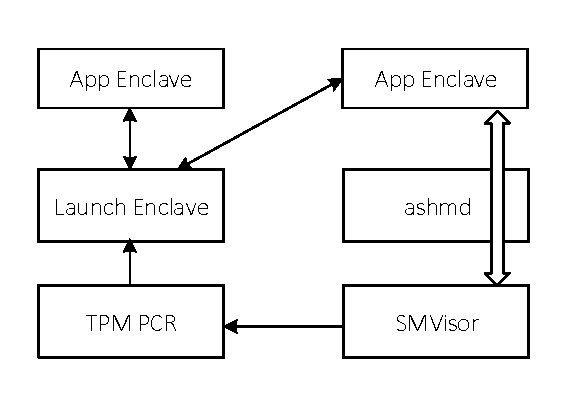
\includegraphics[width=0.3\textwidth]{figures/mutual.pdf}%height=0.2\textheight,
\caption{Mutual attestation and key agreement between SMVisor and an application enclave. The single line arrows denote the attestation direction, the double line arrow denotes the following key agreement.}
\label{fig:mutual}
\end{figure}

\textbf{Mutual Attestation.}
During a measured boot, Intel Boot Guard~\cite{ruan_platform_2014} hashes the firmware and stores its cryptographic hash in the TPM Platform Configuration Register (PCR) \cite{tcg_trusted_2014}. The final PCR value reflects the whole boot process. If the process is tampered with, the PCR value will differ. In order to ease SMVisor attestation, we use the launch enclave provided by the Intel SGX Platform Software to attest SMVisor for one-time effort. Afterwards, any application enclave running on the same machine can query the launch enclave to know if SMVisor attestation has succeeded. To attest  SMVisor, the launch enclave needs to verify the PCR value by requesting a TPM quote, which includes a cryptographic signature over the PCR value alongside with a fresh nonce. This ensures the integrity of the PCR value and prevents replay attacks. Besides, an application enclave attests itself to the launch enclave using Intel's local attestation.

\textbf{Key Agreement.}
After the mutual attestation, the SMVisor and an enclave establish an authenticated secure channel via an ephemeral Diffie-Hellman key exchange. We then use AES-GCM encryption scheme for further message exchange in order to prevent replay attacks. Intel processors with SGX feature support Advanced Encryption Standard New Instructions (AES-NI) to accelerate AES encryption and also can mitigate side-channel attacks~\cite{Corporation2016Intel}.

%\subsubsection{Communication}
%% 通信要依赖共享内存,在此基础上设计协议
%We design a protocol for message exchange between SMVisor and enclaves in a secure session.

%\textbf{Communication Protocol Interface.}
%%% 协议接口说明,关于EnclaveID看是用什么好,EPID拿不到的话
%Aurora proposes a uniform abstraction interface between Tlibaurora and SMVisor: \textit{IOCTL(DEVICE, ENCLAVEID, OPERATION, PAYLOAD)}. The first argument indicates the device that an enclave desires to communicate with. The second distinguishes the identity of requestor; an ENCLAVEID can be obtained using \textit{EREPORT} instruction. The third stands for the operation type to be performed, it can be either of the three: PROBE, READ and WRITE. The last argument carries the message data. All the arguments are marshaled and encrypted into the secure channel.  

\textbf{Termination.}
%% 和进程退出释放资源一样,我们这个并不老是影响系统
When an enclave finishes its requests, its Tlibaurora logic will notify SMVisor to terminate the secure session and release resources. When there remains no live session, SMVisor will disable its interrupt routing and thereafter make no impact on the system.

\subsection{Security Enhancement and Performance Optimization}\label{enhancement}
To provide better security and performance, \textsc{Aurora} introduces \textit{hardware encryption}, \textit{data obliviousness} and \textit{batch mechanism for smcalls}.

%% 硬件加速效果如何
\textbf{Hardware Encryption.}
Intel extends x86 ISA with AES-NI and claims to prevent known side-channel attacks. We make use of it to address the same concern and use a constant-time AES-128-GCM algorithm to defeat cache timing attacks. Nonces are used for replay proof. This hardware accelerated encryption also decreases the preemption time in SMM.

%% 数据隐藏,保证每次内容的随机性
\textbf{Data Obliviousness.}
In an established session, if an enclave requests the same I/O path twice and the results happen to be the same, the encrypted messages will also be identical because the session key is not changed. An adversary can infer secrets by observing such side channels. To prevent such secrecy leakage, \textsc{Aurora} pads all messages with random values to the same length (4KB, same size as one EPC page), which restricts possible information leakage at page-level. The maximum length of a message is 4080 Bytes, leaving at least 16 bytes for random padding.%The message buffers must start with page-aligned address.

\textbf{Batched SMCALLs.}\label{batch}
To reduce the context switches between SMVisor and enclaves, \textsc{Aurora} supports a batched \textit{smcalls} mechanism using two dedicated, lock-free ring buffers for input and output respectively. %It is especially useful in the case of highly frequent requests.
Enclaves can set a desired threshold, so Tlibaurora will coalesce these \textit{smcalls}. For asynchronous I/O requests, the mechanism can benefit the enclave with higher throughput.


\section{Trusted I/O Paths between Enclaves and Devices}\label{tpaths}

As described in section~\autoref{types},  trusted I/O paths  should assure that the users' data is transferred by a secure session. 
%The fundamental reason is that these devices can only understand data in plaintext form. To defeat eavesdropping attacks, the data is encrypted and sent through the secure session. Until it reaches the SMRAM will the encrypted data be decrypted into the clear text, so the untrusted system is unaware of the operations that SMVisor has performed to the target devices. 
In this section, we illustrate how to build trusted I/O paths for data-provider/consumer devices, e.g. human-interface-device (HID) keyboards, serial printers, and hardware clocks, and data-storage/transmitter devices, e.g. portable USB disk.

\subsection{Trusted HID Keyboard Input}\label{input_service}
Trusted input ensures that third-party software on the same computer has no access to the user's input intended for an enclave application. In other words, trusted input paths exclude other untrusted software including the underlying OS from sharing the input device. We use \textsc{Aurora} to secure user's private textual inputs from the keyboard to the enclave.%, and SGX perfectly secures the input inside the enclave.

\textbf{Trusted Input Mode.}
When an enclave issues a trusted input request, SMVisor routes the keyboard interrupt (IRQ 1 by default) to SMI. All of the subsequent keyboard scan codes are then cached inside SMRAM. We call this case \emph{trusted input mode}. After an \emph{enter} key is hit and released, SMVisor recovers the I/O APIC redirection table and exits trusted input mode. Finally, SMVisor encrypts the input and sends it to the secure channel. The desired enclave obtains it from the channel and decrypt it.

\textbf{User Verification.}
%Phishing attacks, where an adversary exploits social engineering tricks to allure a user to leak her privacy data, are a threat to trusted input. For example, a malware might present a fake login interface that prompts a user to enter her password.
Attackers can use keyloggers to steal passwords or credit card information. Most keyloggers are not stopped by HTTPS encryption which only protects data in transit between computers. For example, they are frequently implemented as rootkits that subvert the operating system kernel to gain unauthorized access to the hardware. 
To mitigate this threat, we leverage the PC speaker to indicate that the trusted path has been established.
When the system first boots, the network is disabled by the SMVisor, and we assume that the loaded kernel is clean due to TPM's measure boot. \textsc{Aurora} asks a user to store a short, arbitrary MIDI-format melody (around 5 seconds) inside SMRAM via a configure enclave, so that every time when a trusted path is set up, the PC speaker will play the melody, and then the network is enabled by the SMVisor. Since the melody is a pre-shared secret only known by SMVisor and the user, it is impossible for the attackers to learn and mimic this process.
% Tlibaurora first generates a random integer $N$ in the interval of [1, 10], and displays the integer number in the screen as a captcha. Tlibaurora sends $N$ to SMVisor. SMVisor blinks the \textit{Caps Lock} LED light for exactly $N$ times. Since the captcha is generated with noises inside the enclave, it is hard for the adversary to mimic the process. %Before the enclave application displays the prompt that awaits the user to enter her password, a controlled computer might have displayed the same content and user directly inputs the secrecy without waiting for the computer to enter trusted input mode. 

\subsection{Trusted Serial Printer Output}\label{output_service}
Shared print services are very common today, by which colleagues in a unit or students in a college print their documents using the same physical machine. Users' private or sensitive data may also be printed using such infrastructures. Malware or compromised systems running on these shared machines can steal these data for malicious purposes like industrial espionage or illegal data acquisition. To mitigate this threat, we build trusted serial-port path for shared print services.

When an enclave requests the trusted printer service, it encrypts the output packet and sends the encrypted packet to SMVisor.  SMVisor receives the packet and decrypts it to plaintext packet. As the packets are usually held with printer-specific format, SMVisor issues the corresponding serial port driver and adds this job into its task queue. Afterwards, SMVisor returns the status code from the printer devices to the enclave end-point.

\subsection{Trusted Hardware Clock}\label{time service}
The integrity and non-forgeability of the clock value is much more vital. In this section, we describe how to extend \textsc{Aurora} for trusted, absolute, high-resolution and attack-aware clock.

%\textbf{Diverse Sources.}
%%% 多源头获取时间,适应不同需求
%\textsc{Aurora} uses multiple clock sources available on x86 platforms, such as programmable interval timer (PIT) and advanced configuration and power interface/power management (ACPI/PM) timer. 

\textbf{Absolute Value.}
%% 绝对时间来自RTC驱动
We use Real-Time Clock (RTC) to provide the absolute wall-clock time (i.e. epoch) for enclaves. To avoid incorrect values due to hardware updating, SMVisor keeps obtaining the RTC values until the last two are consistent. After obtaining a valid wall-clock, SMVisor then obtains the rest timers. The order is critical because RTC time retrieval is the most expensive amongst others and will break the freshness of other timers' values.

\textbf{High Resolution.}
%% 根据时钟频率和差值计算时间精度
When a time value with high resolution (e.g. micro-second) is required, \textsc{Aurora} uses invariant time stamp counter (TSC) and High Precision Event Timer (HPET). For instance, \textsc{Aurora} uses the following formulae to compute the \textit{tv\_usec} value in \textit{timeval} data structure: {$tv\_usec = (HPET\_value/ HPET\_Hz) / 1,000,000$;} where $(HPET\_value / HPET\_Hz)$ computes the absolute time in micro-seconds. SMVisor references invariant TSC to estimate the latency of hardware response and adjust the value. Invariant TSC ensures that the duration of each clock tick is uniform. 

\textbf{Attack-Awareness.}
%% 如何避免时钟攻击
Though hardware clocks can be controlled and modified by the malicious OS, diverse timers in Aurora offer enclaves the ability to validate the credibility of time values. Tlibaurora records last values read from all hardware clocks and obtains current values to calculate their differences respectively, and then uses clock frequencies to compute the actual elapsed time. When any of the measured time violates the monotonic rule, we assume a time attack.

For the case where the hardware clocks are altered in a consistent way, that is, all the timers are altered in the same offset, we propose a novel algorithm to detect such an attack. We use a dedicated counting thread \cite{DBLP:conf/dimva/SchwarzWGMM17} guarded inside an enclave occupying a logical thread on the same CPU core. Such a sibling thread will block the possibility of side-channel attacks when hyper-threading is active \cite{DBLP:conf/sp/ChenWCCZWLL18}. The counting thread provides $dT$ and the difference of hardware timers provides $dt$, we use first-order derivative $dt/dT$ to detect the possible time attack. Currently, we set the confidence interval to 0.05, which denotes the possible altering in the timers' rising slope. If the slope changes much, we assume an attack.

Aurora's trusted hardware clock is immune to the TOCTOU attack because it leverages SMM which guarantees that the operations of check and use are atomically performed.

\subsection{Trusted USB Storage}\label{storage_service}
Storage software usually supports block devices and file system. A compromised OS may silently discard data written by the application or return fabricated data during a read operation. It is a serious issue when secure data storage is  necessary for ensuring correct operation (e.g., secure logging, APT monitoring and compliance). We extend \textsc{Aurora} to support secure USB massive storage devices as an example. We believe that \textsc{Aurora}'s approach is suitable to support other storage systems such as SATA HDD, NVMe SSD, etc.

% 对于不关注隐私的可信路径,我们主要是利用中断来判断读写的请求。因此每次都显式调用fsync;另外,最大的问题在于如何找到DMA高速缓存区域。
%\textbf{Basic USB Workflow.}
%A USB host controller (UHC), consisting of several physical USB ports, is connected to one USB endpoints.  A UHC is controlled via a set of memory-mapped I/O (MMIO) registers and presented as a PCI device in an OS, which uses a USB Host Controller Driver (UHCD) to communicate with it. %to issue request packets defined by the specific UHCD. % These contain a number of pointers to various linked lists that track attached devices and map requests to devices.  %A higher-level device driver communicates with the specific endpoint device via the HCD and hardware. 
%We take an EHCI device in Linux as an example, its device driver sends a USB request block (URB) to query information from the device. The UHCD creates a transfer descriptor (TD) for this request and links it to a list \textit{reqlist} for the device. Once this request is completed, the UHC will unlink the TD from \textit{reqlist} and link it to a \textit{donelist}. It also writes result data into memory via DMA and sends an interrupt indicating it has new data on \textit{donelist}. On receiving this interrupt, the UHCD walks \textit{donelist} and processes the TDs found. It then notifies the device driver (typically via an asynchronous callback) that its URB is serviced and the data is available.

\textbf{Secure Storage Protocol.}
%The IRQ number of the device is acquired by ashmd module and then notified from ashmd to the underlying SMVisor. 
When an enclave issues a request for a USB storage device, SMVisor leverages I/O interrupt rerouting mechanism to monitor and deal with every operation of the USB device, including transferring data and control commands via a secure session in \textsc{Aurora}. In Linux, the data is by default transferred using bulk mode and is exchanged based on DMA mechanism, which stores the DMA address and buffers location in a {scatter-gather} list. The ashmd module obtains the information from the USB driver.

% 描述了基本的协议,保证每次读写请求都能得到SSV的确认
%% 无法使用S2BR的设计,因为没有维护任何文件名和文件大小的基本信息,我们无法以文件作为MAC完整性检查的基本单位
After capturing the USB Request Blocks (URBs), SMVisor passes them to the USB device via a secure session.  Note that SMVisor leverages AES-GCM scheme to encrypt transferred blocks between enclaves and devices \ref{arch}. All data blocks from the enclave are encrypted by default, and a message authentication code (MAC) is generated for each block. SMVisor checks the MAC of each block to validate its authenticity and integrity. If it checks an inconsistent MAC, SMVisor will return an error to the enclave.

\section{Implementation}

\subsection{Components}

We modified the SMI handler of CoreBoot to implement \textsc{Aurora}'s SMVisor, and modified the drivers of CoreBoot project to export interfaces which can be invoked by SMVisor. We disable the caching mechanism in SMM and check the access permission using the memory type range registers (MTRR) to ensure SMVisor's protection. For the sake of compatibility, Tlibaurora supports standard
POSIX APIs, so enclave developers need not write OCALLs.

To avoid machine check exception within SMM, we enable the Streaming SIMD Extensions (SSE) bit in control register CR0. With SSE and AES-NI, we boost encryption performance. For example, with AES-NI support, AES-256-GCM encryption and decryption on 4KB data in SMM costs 9us on average, for comparison,  without AES-NI, AES-128-GCM implementation of Intel IPP Crypto library~\cite{Intel_IPP_2017_Update_2} costs 597us.

We implement a specific kernel model ashmd. Like Linux SGX driver, we use but do not trust them. The ashmd module is intended to relay the communications between enclaves and SMVisor.

%% 强调TCB小
\subsection{Trusted Computing Base}\label{codebase}
%% 说明移植的轻松程度,强调运行时占据物理内存的少
%We use SLOCCount\footnote{https://www.dwheeler.com/sloccount} to calculate the overall C Lines of Code (LoC) of current \textsc{Aurora} implementation. As shown in \autoref{code_base},  \textsc{Aurora}'s TCB (3393 LoC) is far less than other architectures (see \autoref{arch_compare}). 
\textsc{Aurora}'s trusted components (i.e., SMVisor, ashmd, Tlibaurora, Cryptography) have 3393 lines of C code, and untrusted component (i.e., Ulibaurora) has 273 lines of C code. %Compared to Wimpy kernel \cite{zhou_dancing_2014} which has 16K lines of code, it is smaller and simpler enough to facilitate formal verification.
To avoid exploitable vulnerabilities, we use static analysis tools, e.g., Clang Static Analyzer\footnote{http://clang-analyzer.llvm.org/index.html}, over \textsc{Aurora}'s code base and fix all found bugs. Besides, as \textsc{Aurora} is quite small and its complexity is obviously lower than that of the formally verified microkernel~\cite{DBLP:conf/sosp/KleinEHACDEEKNSTW09}, we believe it is reasonable to put \textsc{Aurora} within reach of formal verification.

On our platform, the system-wide EPC limit is approximately 93MB and the SMRAM is 4MB by default. Both are scarce memory resource. We therefore measure the final size of the resulted stripped binary images. Our modification on CoreBoot only adds 3.9\% on its total size (120.2KB V.S. 115.7KB). The enclave.so  linked against Tlibaurora is 696KB in size and 1MB including runtime stack and heap manager. Smaller codebase denotes smaller TCB introduced. 

%\begin{table}[t]
% \centering
%  \caption{The code base of \textsc{Aurora}}
% \label{code_base}
%\begin{tabular}{ llr }
% \toprule
%& Component & Lines of Code \\
% \midrule
% \multirow{4}{*}{Trusted} &  SMM Supervisor & 274 \\
%& ashmd module & 159 \\
%& Tlibaurora & 1841 \\
%& Cryptography & 1119 \\
%% \midrule  TCB & 3234 \\
% \midrule %\midrule
%Untrusted & Ulibaurora & 273 \\
% \midrule
%TCB/Total & & 3393/3666 \\
% \bottomrule
%\end{tabular}
%
%\end{table}

\subsection{Limitation}
Although SMM-based mechanism can be used to route many peripheral I/O events, it itself cannot be used to protect the framebuffers and therefore fails to provide a trusted display. This is because SMRAM area by default starts at the same address as the VGA space, therefore SMVisor cannot obtain the framebuffer. It can be solved by redirecting  SMRAM to another higher memory area without overlaying the VGA space. However, as SMM-based protection has performance implications~\cite{DBLP:conf/iiswc/DelgadoK13}, we recommend that users choose Intel PAVP (assisted by Intel ME) and SGX~\cite{DBLP:conf/isca/HoekstraLPPC13} for real-time scenarios such as video chattings or conferences.


\section{Evaluation}\label{performance}

In this section, we evaluate the performance of \textsc{Aurora} framework and the trusted I/O paths. Our experiments are carried out on  an Intel Core i7-7700HQ 2.8GHz CPU with 16GB of memory, running Ubuntu 16.04 LTS and SGX SDK 2.4 and SGX driver 1.9.

\subsection{Framework Overhead}

\begin{table}[t]
	\centering
	\caption{Measuring \textsc{Aurora}'s overhead by calculating Pi.}
	\label{table:pi}
	\begin{tabular}{rrrrr}
		\toprule
		\multirow{2}{*}{\textbf{Interval}} & \multicolumn{2}{c}{\textbf{Time cost (s)}} & \multicolumn{2}{c}{\textbf{Overhead ratio}} \\\cmidrule{2-3}	 \cmidrule{4-5}
		& 70us & 150us & 70us & 150us \\
		\midrule
		Baseline & 8.545 & 8.635 & 0 & 0\\
		1000ms & 9.045 & 9.025 & 5.85\% & 4.52\%\\
		100ms & 9.605 & 9.590 & 12.40\% & 11.06\%\\
		10ms & 10.180 & 10.455 & 18.90\% & 21.08\%\\
		\bottomrule
	\end{tabular}
\end{table}

%% 我们使用pi计算做评估,不同触发周期和抢占时间
We select  pi\_css5\footnote{http://myownlittleworld.com/miscellaneous/computers/piprogram.html} program, which has no interaction with the external system, to measure the performance of \textsc{Aurora} with as little noise as possible. We ran the program till achieving 4,000,000 digits of precision, and used two durations (70us and 150us) to emulate different real-world environments.

%% 一个线程触发,一个线程计时
%% 太高的请求我们认为不合理;OS有权拒绝SMI请求,以此降低性能影响
Specifically, we ran two threads: one thread (T1) running Pi number calculation, the other thread (T2) requesting the ashmd module to trigger an SMI in a given interval. Firstly, we ran T1 without the interference of T2 and took the time cost as a baseline. Then we started T2 to see the slowdown of T1. From \autoref{table:pi}, we observe that when the interval decreases, the overhead increases. The worst case of overhead is around 21\%, where \textit{smcalls} are requested too frequently. Such a situation is rare in real world applications because an enclave has to execute its own logic. We observe that intensive requests may impact the time-sensitive tasks on the same system. Since \textit{smcalls} are forwarded by ashmd module, it can use a threshold to block a malicious enclave from abusing. In our current setting, we allow an enclave to request up 10,000 times per second, which introduces about 11\% overhead to the system.

\subsection{Security Evaluation}\label{security}
We evaluate \textsc{Aurora}'s reliability with several security tests.
\\
\textbf{Keylogging Attack.}
To evaluate the effectiveness of \textsc{Aurora}'s trusted input path, we deployed multiple spyware to get a user's inputs under trusted input mode, including a stealthy root keylogger\footnote{https://github.com/vim2meta/keylogger}, a rootless X11-based keylogger ixkeylog\footnote{https://github.com/dorneanu/ixkeylog}, a kernel-level rootkit keylogger\footnote{https://github.com/arunpn123/keylogger}, and a remote keylogger\footnote{https://github.com/EinBaum/Totally-Not-A-Virus}. None of them can obtain the user's inputs.
\\
\textbf{Output Corruption Attack.}
We leveraged a DMA-based NIC device to launch output corruption attack when using Aurora's trusted serial printer service. Since  SMRAM and EPC RAM are strongly isolated by architectural protections, only meaningless content (0xFF) is obtained. No secrets are leaked. We then conducted another DMA attack to corrupt SMM drivers outside of SMRAM. SMVisor detected its integrity tampered  and rejected subsequent requests, then notified the enclave application. Moreover, we conducted another DMA attack to corrupt the content of shared memory of the secure session. Both SMVisor and Tlibaurora can verify the broken MAC and restart a new session.
\\
\textbf{Time Deception Attack.}
To evaluate the trusted clock, we intentionally modified the RTC when an enclave issued a request for trusted clock. Tlibaurora detected the attacks successfully and indicated a failure. For instance, \texttt{gettimeofday()} returns -1 and sets the global variable \textit{errno} appropriately. Existing C library specification does not have a flag indicating time attacks, the enclave logic may keep requesting until obtaining a valid time value. We support failure handling in Tlibaurora to help enclaves deal with such situations.
\\
\textbf{Storage Deception Attack.}
We modified the kernel driver of SCSI device and randomly dropped several disk I/O requests intentionally.  SMVisor detected such accidental conditions and notified the Tlibaurora of corresponding enclave. In our current setting, the Tlibaurora will automatically try issuing the lost I/O requests three times so as to avoid storage failure. In our experiments, the enclave finally received the attack warning from the Tlibaurora and logged these events for further forensic analysis. Note that denial-of-service to Aurora's kernel module is not considered in this work.


\begin{table}[t]
	\centering
	\caption{Serial-port benchmark comparison between Linux and \textsc{Aurora}.}
	\label{table:serial}
	\small
	\begin{tabular}{lrrr}
		\toprule
		\textbf{Payload Size(KB)} & \textbf{Linux(s)} & \textbf{Aurora(s)} & \textbf{Speedup(\%)} \\
		\midrule
		4 & 0.03 & 0.03 & 0.0 \\
		64 & 0.32 & 0.24 & 25.0 \\
		256 & 1.08 & 0.87 & 19.4 \\
		1024 & 3.95 & 3.43 & 13.2 \\
		\bottomrule
	\end{tabular}
\end{table}

\begin{table}[t]	
	\centering
	\caption{Storage throughput comparison between Linux and \textsc{Aurora}.}
	\label{table:dd}
	\small
	\begin{tabular}{lllr}
		\toprule
		\multirow{2}{*}{\textbf{Payload Size(MB)}} & \textbf{Linux} & \textbf{Aurora} & \textbf{Slowdown} \\ 
		& \textbf{(MB/s)} & \textbf{(MB/s)} & \textbf{(\%)} \\
		\midrule
		4 & 32.9 & 31.8 & 3.3 \\
		64 & 40.9 & 39.2 & 4.2 \\
		256 & 42.7 & 40.4 & 5.3 \\
		1024 & 53.2 & 47.5 & 10.7 \\
		\bottomrule
	\end{tabular}
\end{table}

\iftrue

\begin{table}
	\centering
	\caption{ Breakdown of the trusted clock service}
	\small
	\label{table:breaktime}
	\begin{tabular}{lr}
		\toprule
		\textbf{Action Step} & \textbf{Time Cost(us)} \\
		\midrule
		EPC encryption & 2\\
		Copy to DRAM & 2\\
		Switch to SMM & 13\\
		Copy to SMRAM & 0\\
		SMM decryption & 3\\
		Clock Service & 44\\
		SMM encryption & 3\\
		Copy to DRAM & 0\\
		Return and enter SGX & 12\\
		Copy to EPC & 3\\
		EPC decryption & 2\\
		\bottomrule
	\end{tabular}
\end{table}

\begin{table*}[t]
	\centering
	\caption{Comparison of existing clock services that can be used for SGX enclaves. Clock services include network time protocol (NTP), precision time protocol (PTP), and the platform software (PSW) supported by Intel management engine (ME), monotonic counter supported by Byzantine Fault Tolerance (BFT) protocol.}
	\label{table:timeservice}
	\small
	\begin{tabular}{lllcrccr}
		\toprule
		\textbf{Clock Provider} & \textbf{Approach} & \textbf{Type} & \textbf{Resolution} & \textbf{Request Cost} & \textbf{Latency} & \textbf{Security} & \textbf{Use Cases} \\
		\midrule
		Remote Clock & NTP/PTP & absolute & 1s & $>$100ms & high & trusted & Town Crier~\cite{DBLP:conf/ccs/ZhangCCJS16} \\
		Intel ME & PSW & relative & 1s & 10.3ms & medium & trusted & SGX-Tor~\cite{DBLP:conf/nsdi/KimHHKH17} \\
		OS Kernel & OCALL & absolute & 1ns & 6us & low & untrusted & Panoply~\cite{shinde_panoply:_2017} \\
		Distributed Network & BFT & N/A & N/A & 1--2ms & medium & trusted & ROTE~\cite{DBLP:conf/uss/MateticAKDSGJC17} \\
		Hardware Clock & \textit{smcall} & absolute & 1ns & 69us & low & trusted & Aurora-OpenSSL~\ref{openssl} \\
		\bottomrule
	\end{tabular}
\end{table*}

\fi

% 测试结果说明Aurora方法下的串口响应速度更快,和Linux原生方法频繁的上下文代价有关
\subsection{Serial Port Output Benchmark}

It is rather difficult to measure the overall time during which a printer accepts and finishes a print job, because we have to re-flash the printer firmware to hook its time function. Therefore, we redirected the serial port to a local file. 
To compare the serial output performance between native Linux and \textsc{Aurora}, we measured the time cost of writing the test data of different sizes to the serial-port address in Linux and in \textsc{Aurora}, respectively. \autoref{table:serial} shows the experimental results. \textsc{Aurora} performs better than native Linux because \textsc{Aurora} uses batch mechanism (\autoref{batch}) to reduce the frequent mode transitions while Linux has more user/kernel mode transitions when writing large data to a serial port. Note that, for the larger output data, the speedup decreases due to cryptographic computations in \textsc{Aurora}.

\subsection{Trusted USB Storage Benchmark}

To compare the overhead introduced when applying \textsc{Aurora}'s trusted I/O path on USB storage devices, we wrote variable sizes of contents to a USB storage device on native Linux system as the baseline, by using \texttt{dd} program with options \texttt{fsync} and \texttt{direct}. To avoid the side-effect of any buffer mechanism, we use Linux raw device to mount and initialize the USB device. % to bypass any file system interference. We then measure the overheads of using Aurora's SMVisor for MAC verification added to each block request in the request and response path. We did not use any encryption in this experiment. 
The throughput results are shown in \autoref{table:dd} where the size of each block is set to 4KB. \textsc{Aurora} achieves approximately 90\% of the baseline throughput when writing 1GB to the device. The major overheads are contributed by SMM/Protected mode transitions and cryptographic computations on each block.

\subsection{Trusted Clock Benchmark}\label{time_bench}

%It is important to quantify how much time is required to attain a trusted clock service since the potential service latency impacts the freshness of message and indicates the response speed. 
For this experiment, we measured the complete trusted clock procedure for 1,000 times and used the average value. Table \ref{table:breaktime} shows the time cost for each step in a trusted clock path. We can see that the clock service takes most of the time. This is because 1) the RTC driver has to read clock value twice to check if the clock is updating its time data; 2) The RTC involves several \texttt{INS} instructions to read each field of a calendar time, and costs 14us to obtain a complete wall-clock time in one request; 3) The other 4 timers cost roughly 10us in sum. The total  time cost (84us) satisfies the requirement of real-world trusted timestamps.

For comparison, we measured the performance of other clock providers. The results are shown in \autoref{table:timeservice}. %Due to the fact that there are no input dependent branches in the secure channel (the channel simply transfers the I/O packets), we argue that our secure session is safe from side-channel attacks such as the timing attacks. 
Among existing approaches, \textsc{Aurora} outperforms remote clock (the 2nd row) and Intel's reference clock (the 3rd row) by introducing very low latency, while achieving the same resolution (nanosecond-level) as OS services (the 4th row). 
%Note that any approach can be arbitrarily delayed in that the untrusted OS is in charge of the enclave thread scheduling. We treat intentionally time delay as a form of Denial-of-Service attack.

\section{Case Studies}\label{casestudy}

Aurora provides uniform abstractions (standard POSIX APIs) for the SGX applications, which need not be modified, to maintain platform-independence and thus achieve nice usability. We implemented trusted I/O paths for three real-world applications to illustrate the usability of \textsc{Aurora}.

\subsection{Secure OpenSSH Login}\label{openssh}

%\begin{figure}[t]
%	\centering
%	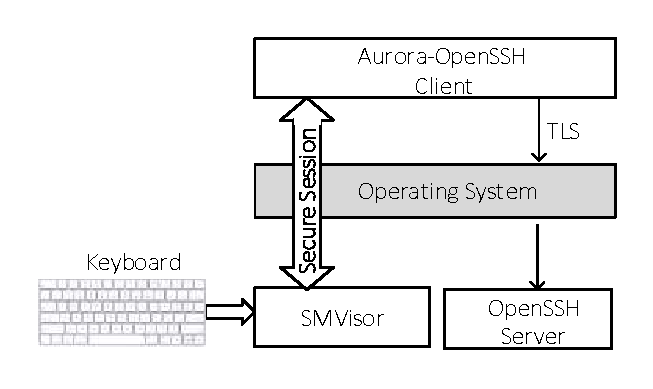
\includegraphics[width=0.4\textwidth]{figures/ssh.pdf} %height=0.16\textheight,width=0.6\textwidth
%	\caption{Aurora-OpenSSH with trusted input path.}
%	\label{fig:openssh}
%\end{figure}

Secure Shell (SSH) is widely used for shell access on UNIX-like systems. An SSH server uses a username and a password to authenticate an SSH client. If the client is infected with malware, the login credential can be stolen by key-loggers. To demonstrate the effectiveness of \textsc{Aurora}'s trusted input path, we modified OpenSSH 7.7 to protect its client login process. Specifically, we ported passphrase related logic into an enclave, and used \textsc{Aurora}'s \textit{trusted input path} to get passwords which users input. We call the enhanced client as Aurora-OpenSSH client. %, as depicted in \autoref{fig:openssh}.

Aurora-OpenSSH client first requests SMVisor to intercept the user's  keyboard events. This interception adds around 13\% overhead per keystroke. Only after SMVisor routes the keyboard interrupt into itself and acknowledges to the client, will the prompt \texttt{"username@hostname password:"}  be displayed on the screen. While the user is typing the passphrase, the client does not display any content on the screen, achieving the same effect as in the native OpenSSH client.

The user's input is buffered inside SMRAM. When the user releases \texttt{Enter} key, the password is then encrypted and sent to the secure channel, and SMVisor exits trust input mode.  Aurora-OpenSSH client reclaims the password message and sends it to the server. Note that the plaintext password is only available in SMRAM and enclave. The path between SMRAM and enclave is protected by \textsc{Aurora}'s secure channel and the path between Aurora-OpenSSH client and OpenSSH server is protected by TLS session.
%
%%Recall that SMVisor will manipulate the LED to blink random times to indicate that it has intervened the keyboard interrupts. Because we use virtualized environment to do the experiments, our current prototype uses serial output to indicate this.

\subsection{Secure OpenSSL Session}\label{openssl}

%\begin{figure}[t]
%	\centering
%	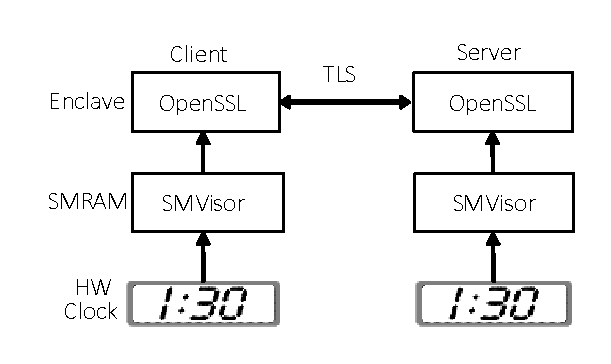
\includegraphics[width=0.35\textwidth]{figures/ssl.pdf} %height=0.2\textheight,
%	\caption{Aurora-OpenSSL with trusted clock.}
%	\label{figure:openssl}
%\end{figure}
%There are multiple in-enclave SSL/TLS project on going \cite{mbedtls, intel_sgx_ssl, wolfSSL}. These projects employ SGX to provide tamper-resistant cryptographic process.
SSL/TLS protocols are in widespread use in web browsing, email, instant messaging, and voice-over-IP, etc. 
%To allow for a distributed communication, a secure session named TLS is established between two parties. 
An SSL/TLS session starts with SSL/TLS handshake protocol, including authentication, key exchange, etc. The procedures rely on system date and time. The SSL/TLS server needs to provide a certificate with a timestamp indicating the expiration time, and the SSL/TLS client needs to verify this certificate. Most of all, both parties require a reliable time source to detect possible timeout. For instance, both \emph{ClientHello} and \emph{ServerHello} messages use the system time to prevent replay attacks. If the time is emulated by an untrusted source, it may compromise the security of OpenSSL sessions.

One of the in-enclave SSL/TLS projects is SGX-OpenSSL\footnote{https://github.com/sparkly9399/SGX-OpenSSL} from SGX-Tor project~\cite{DBLP:conf/nsdi/KimHHKH17}. It does not trust the system storage, therefore its server side creates the certificate inside the enclave each time it receives a new connection request from the client side. We enhanced the TLS handshake by using \textsc{Aurora}'s trusted clock. Specifically, we replaced time-related OCALLs in the original project with \textsc{Aurora}'s libaurora. %The new architecture of TLS handshake is demonstrated in \autoref{figure:openssl}.
We measured the time cost of certification generation at server side and TLS handshake at client side for 10,000 runs and take the average value. We also measured the native SGX-OpenSSL using original OCALLs. As shown in \autoref{table:openssl}, in our LAN setting, Aurora-OpenSSL introduced about 32\% latency in certificate generation and 21\% in the TLS handshaking because both of them use \textsc{Aurora}'s trusted clock. We anticipate the overhead ratio to decrease in a WAN environment, because the delay of a geographically distributed public network should be larger than our LAN setting.

%\subsection{Secure Online E-Banking}
%
%\begin{figure}[t]
%	\centering
%	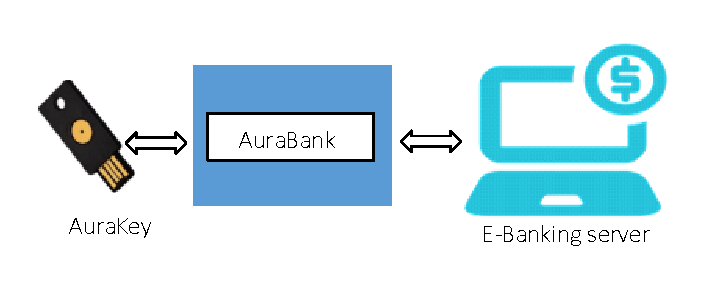
\includegraphics[width=0.45\textwidth]{usbkey.pdf} %height=0.1\textheight,
%	\caption{AuraKey with trusted USB path}
%	\label{fig:usb}
%\end{figure}
%
%State-of-the-art secure token mechanism employs a two-factor authentication, which combines a user password and a physical device (usually a USB key, e.g. Yubikey\footnote{https://www.yubico.com/products/yubikey-hardware/yubikey4/}). %that provides digital certificate to prove genuine user identity. One of the popular examples is Yubikey\footnote{https://www.yubico.com/products/yubikey-hardware/yubikey4/}. Because these USB key implementations are not open source, we built a secure E-Banking application according to their documentation. We name our USB key and secure E-Banking implementation as \textit{AuraKey} and \textit{AuraBank} respectively.
%Typically, a USB key identifies itself as a USB HID keyboard device so that any machine with a keyboard driver can easily read the textual outputs from it, therefore, we use an EHCI-based USB HID keyboard to emulate a USB key, named \textit{AuraKey}. We created an enclave program as a hardened E-Banking prototype, named \textit{AuraBank} and equipped \textit{AuraKey} with a PKCS format certificate from \textit{AuraBank}, as shown in \autoref{fig:usb}. We wrote a script to attach/detach the USB device during runtime, emulating the action of plugging/unplugging of \textit{AuraKey}. We deployed the server side of \textit{AuraBank} on a standalone machine in the local area network.
%
%We then illustrate how Aurora-assisted online E-Banking works. Firstly, a user launches the \textit{AuraBank} application and then performs some personal transactions. All of the confidential transaction logs are locally cached within the enclave of the \textit{AuraBank}. When the user commits her transactions to the bank server, she needs to hot-plugin the \textit{AuraKey} to confirm her operations. After being inserted into the USB slot, the \textit{AuraKey} triggers an SMI to notify SMVisor, which then intercepts all input interrupts of \textit{AuraKey} and obtains the security token. SMVisor hands the security token to \textit{AuraBank} via secure channel. Finally, \textit{AuraBank} sends transaction data and identity authentication information to the bank server via TLS protection, which then authenticates the user identity and validate her transaction. %with what the user knows (i.e. the personal identification number a.k.a PIN) and what the user has (i.e. physically secured private key).
%
%\begin{table}[t]
%	\centering
%	\caption{Aurora-secured Online E-Banking Benchmarks}
%	\label{table:usbkey}
%	\small
%	\begin{tabular}{lr}
%		\toprule
%		Procedure & Time Cost (ms) \\
%		\midrule
%		AuroKey -> AuroBank & 0.468  \\
%		AuroBank -> E-Banking server & 28.701 \\
%		\bottomrule
%	\end{tabular}
%\end{table}
%
%The experimental results are shown in \autoref{table:usbkey}. The first procedure contains the private data transferring from the physical device (AuroKey) to the userspace software (AuroBank); the token is transferred via the secure session with AES-NI based cryptographical protection. The second procedure contains the encrypted two-factor information with TLS protection between two machines. Since the TLS session usually takes 10~ microseconds or more, Aurora's two-factor adds negligible overhead to the authentication process. With the help of trusted path, it is impossible for any untrusted software on the user computer to access either USB token or user password. % or other local credentials. %An alternative would be the OTP (one-time password) device that allows the user to login without remembering any password. The OTP device can also be secure using Aurora's framework.

\begin{table}[t]
	\centering
	\caption{Performance comparison between native SGX-OpenSSL and Aurora-OpenSSL.}
	\label{table:openssl}
	\small
	\scalebox{0.8}{
	\begin{tabular}{lrrr}
		\toprule
		& \textbf{SGX-OpenSSL} & \textbf{Aurora-OpenSSL} & \textbf{Slowdown(\%)}\\
		\midrule
		{Certificate Generation} & 77.4ms & 102.5ms & 32.4\\
		{TLS Handshaking} & 2.8ms & 3.4ms & 21.4 \\
		\bottomrule
	\end{tabular}}
\end{table}

\begin{table}[t]
	\centering
	\caption{TPC-H benchmark comparison between native SGX-SQLite and \textsc{Aurora}-SQLite.}
	\label{table:tpch}
	\small
	\begin{tabular}{lrrr}
		\toprule
		\textbf{Query} & \textbf{SGX-SQLite(s)} & \textbf{Aurora-SQLite(s)} & \textbf{Slowdown(\%)} \\
		\midrule
		02 & 4.68 & 5.10 & 8.97 \\
		11 & 1.29 & 1.42 & 10.08 \\
		16 & 1.08 & 1.10 & 5.30 \\
		17 & 91.26 & 93.30 & 2.23 \\
		18 & 24.98 & 25.91 & 3.72 \\
		19 & 93.15 & 98.25 & 5.47 \\
		21 & 39.68 & 43.16 & 9.04 \\
		\bottomrule
	\end{tabular}
\end{table}

\subsection{Secure SQLite Database}
Databases are widely used to store financial transaction records and other sensitive information. Some databases are built upon block devices, while maintaining its own caching mechanisms and storage policies without support of OS's file system, e.g. SQLite database.

We integrated \textsc{Aurora}'s Tlibaurora into existing SGX-SQLite projects\footnote{https://github.com/yerzhan7/SGX\_SQLite} and added code to support standard file system calls such as \textit{open}, \textit{read}, \textit{write}, \textit{stat}, \textit{lstat}, \textit{fstat}, \textit{fsync}, \textit{fcntl}, \textit{ftruncate} and \textit{unlink}. We then eliminated the file-related OCALLs from the untrusted system. 
To protect the data, Tlibaurora's shim layer uses a symmetric key derived from user password and in-enclave nonces to encrypt the file payloads. %, and computes MAC values for blocks. 
To avoid password leak, we use \textsc{Aurora}'s trusted input path to obtain users' passwords from keyboard devices. Moreover, \textsc{Aurora}'s secure session protects the confidentiality and integrity of data between SQLite enclaves and SMVisor.
When SQLite invokes Tlibaurora file APIs, it opens the USB storage device in direct I/O mode and reads/writes data using 4KB block size. 
Finally, we set the synchronize flag to \texttt{FULL} to avoid the uncertainty of I/O caching.

We evaluated the enhanced SQLite performance by running standardized TPC-H benchmark\footnote{http://www.tpc.org/tpch/} over a large database. These queries include \textit{select from, order by, group by} benchmarks. % (around 1.3GB).
We make minor changes to these query scripts to make them possible to be executed in SQLite. 
%In our experiment, the native insertion transactions for 1000 times cost 17.3 seconds while the ones with \textsc{Aurora}'s trusted path cost 20.5 seconds. About 18\% overhead is introduced because of the extra encrypt/decrypt computation and mode transitions in \textsc{Aurora}.
\autoref{table:tpch} shows the completed queries\footnote{Note that not all queries can be executed due to the partial porting of the original project.} and their results of native SGX-SQLite and \textsc{Aurora}-SGLite respectively. In our experiments, no more than 10.08\% overhead is introduced because of the extra encrypt/decrypt computation and mode transitions in \textsc{Aurora}.
Note that these are the worst-case overheads (because we have set \texttt{PRAGMA synchronous} to \texttt{FULL}) as almost all databases have their own optimized caching mechanisms for better performance.

%\subsection{Secure Password Manager}
%To ease the cumbersome memoir on multiple passwords, password manager is a convenient tool that allows the end-user to store and manage her passwords. It uses a master key to encrypt the rest of password in a local database. %Though convenient, it may still be vulnerable and render user critical information at risk. An advanced malware can hook the activity of the password manager application and log the corresponding the key events when a "new entry" GUI window is popped up, compromising the security of user password.
%Intel's SGX tutorial \cite{HoekstraUsingInnovativeInstructions2013} uses a password manager to demonstrate the usage of SGX. %Indeed, Intel SGX is a perfect technology for protecting the password manager software itself at runtime as well as the password processing process. 
%However, a user still needs to type in his username and password to initialize a password entry. Without a trusted input path, the SGX-assisted password manager cannot assure to protect the user's confidentiality.
%
%We retrofitted KeePassX, an open source GUI password manager, to demonstrate Aurora's trusted input path. We ported the crypto process, kdbx password database and entry editing functions into an enclave program, so that the user's passwords are clear text only in the enclave. When the user adds a new entry, a GUI message box is popped up, and SMVisor is activated to intercept all keyboard inputs. %Since the GUI logic is untrusted, we do not allow the GUI to touch the real password character, rather, after the user releases a key, the enclave sends the \textit{signal} to GUI and the GUI displays an asteroid. 
%After the user clicks the "OK" button, her username, password and other private information are then encrypted inside the enclave, and later restored into the database in an encrypted format.

\section{Related Work}
Our technique was inspired by Scotch~\cite{DBLP:conf/raid/LeachZW17} which is the first work that combines SGX and SMM to audit VM resource usage. Its motivation differs from ours.
Similar to \textsc{Aurora}'s SMVisor, previous research efforts such as HyperCheck~\cite{DBLP:conf/raid/WangSG10}, HyperSentry~\cite{DBLP:conf/ccs/AzabNWJZS10} and IOCheck~\cite{DBLP:conf/esorics/ZhangWLS14}, also employ a dedicated SMI handler to protect the integrity of the OS kernel, hypervisor or firmware, respectively.
We next discuss related work of other trusted I/O architectures and trusted paths.

\subsection{Trusted I/O Architectures}

SGXIO~\cite{weiser_sgxio:_2017} discusses how to provide trusted generic I/O paths for SGX enclaves. It introduces a trusted hypervisor to assist the establishment of the trusted path, and requires users to port drivers into enclaves. However, SGXIO is a conceptual design without any implementation and evaluation. It is hard for users to port commodity drivers into an enclave because 1) enclave mode does not support privileged instructions; 2) it is unclear how to partition drivers. In contrast, \textsc{Aurora}'s drivers are invoked in SMM with no instruction restricted. Drivers are regulated by SMVisor protected inside SMRAM. This reusing technique allows \textsc{Aurora} to be deployed easily.

Zhou et al.~\cite{zhou_dancing_2014} introduce a microhypervisor named Wimpy to build trusted paths between a program  and a device. This work requires the program to contain the driver associated with the device. It admittedly claimed that running drivers in user model (Ring 3) is difficult. \textsc{Aurora} and Wimpy share many common security goals, e.g. interrupt isolation and MMIO protection. \textsc{Aurora} has smaller TCB than Wimpy. 

Intel platform services (PSW)~\cite{intel_psw} provisions trusted time and monotonic counters by running a coprocessor (Intel Management Engines). It brings separated hardware (e.g., NIC, RTC and SPI flash) that cannot be controlled by untrusted host system. However, since Intel ME runs concurrently with host CPUs, it is difficult and insecure to implement secure human-interface inputs as \textsc{Aurora} does; the host CPUs controlled by untrusted OS and the ME coprocessor controlled by trusted firmware will race a DMA access to the keyboard buffer, which may corrupt or leak user's confidential input. By contrast, \textsc{Aurora}'s SMVisor in nature preempts the untrusted OS.

\subsection{Specific Trusted Paths}

\textbf{Trusted Input Paths.}
On the desktop side, TrustLogin~\cite{zhang_trustlogin:_2015} uses SMM to protect user passwords. It caches the password inside the SMRAM; when the user releases the \texttt{Enter} key, TrustLogin places the password inside the packets of the NIC buffer. In contrast, \textsc{Aurora} does not need to intercept OS networking services, thus decreasing overall impact surfaces.
Fidelius \cite{DBLP:journals/corr/abs-1809-04774} leverages a Raspberry Pi to implement a secure channel between a keyboard and a hardware enclave. The specific LED is turned on when the secure channel is established.  \textsc{Aurora} does not need any specialized I/O devices and reuse existing hardware devices.
On the server side, SafeKeeper~\cite{DBLP:conf/www/KrawieckaKPMA18} leverages SGX to protect the password databases on untrusted clouds. It uses several strategies to mitigate attacks such as phishing. As Intel SGX is also available on personal laptops and mini PCs (i.e., NUCs), we take advantage of SGX to protect a use's password when he logs in his client computer, which differs from their scenarios.
On the mobile side, TrustUI~\cite{DBLP:conf/apsys/LiMHXZCL14} exploits ARM TrustZone to build a trusted path between a user and a service provider, because ARM TrustZone can isolate physical memory and peripheral interrupts. In design, SMVisor is similar to the trusted OS inside TrustZone's secure world.

\textbf{Trusted Clock Paths.} Intel PSW~\cite{intel_psw} supports coarse-grained trusted time but does not provide a wall-clock time. \textsc{Aurora} provides high resolution and absolute clock. ShieldBox~\cite{DBLP:conf/sosr/TrachKGABF18} achieves high-precision yet low-latency clock service by on-NIC PTP clock, however, the time source is not secure because enclaves cannot detect if NIC-Timer is tampered. By contrast, \textsc{Aurora} can detect time attack via a validation algorithm. Déjà Vu~\cite{DBLP:conf/ccs/ChenZRZ17} implements a reference clock thread using transactional synchronization extensions (TSX) to protect a trustworthy source of time measurement. Déjà Vu's goal is to detect interrupt-based attacks, while \textsc{Aurora} can provide a general time service for enclaves. Compared to our prior work \cite{DBLP:conf/eurosys/LiangL18}, which provides a trusted clock to enclaves, \textsc{Aurora} proposes a unified framework for different I/O devices and presents more evaluation on real-world applications. For distributed enclaves, ROTE~\cite{DBLP:conf/uss/MateticAKDSGJC17} proposes a protocol to provide a monotonic counter, which has high latency than \textsc{Aurora}'s trusted clock service.

\textbf{Trusted Storage Paths.}
AuditedIO \cite{DBLP:conf/apsys/BalakrishnanCBS17} leverages SGX and a kernel module to implement verifiable data storage for disk I/O operations. It requires a programmable SSD device and modifies the firmware.
By contrast, \textsc{Aurora} aims for a trusted-path framework which can be used to support general storage devices. % and it protects SMM supervisor inside SMRAM and use mutual authentication to ensure its authenticity.
Jang~\cite{Jang2017Building} builds a trusted path between a USB proxy device and an enclave. The proxy device uses LED display for user verification. It plays the role of  \textsc{Aurora}'s SMVisor while \textsc{Aurora} does not need to introduce dedicated hardware. % while meeting the same or better protection requirements.
BASTION-SGX~\cite{DBLP:conf/isca/PetersLVPK18} modifies the Bluetooth firmware and establishes trusted paths between Bluetooth devices and enclave programs. It has a similar threat model with \textsc{Aurora} and rules the privileged software (OS, drivers, etc.) out of the TCB. %However, it requires enclave programs to take charge of handling the HID input, which is a burden for developers. % and outstands BASTION-SGX by its high extensibility. It is a client/server architecture whereas Aurora reuses existing hardware features on one machine.% light-weight terminal on the end-host to,  Bumpy~\cite{DBLP:conf/ndss/McCunePR09} utilizes dedicated hardware to establish trusted user input path and hence cannot generalize to other devices. Cloud Terminal~\cite{DBLP:conf/usenix/MartignoniPZHMSPPSS12} is a micro-hypervisor-based method that provides terminals secure access to sensitive applications from an untrusted OS. 
Pesos~\cite{DBLP:conf/eurosys/KrahnTVKBF18} builds a trusted path between enclaves and cloud-based storage, and supports policy-based object protection. Still, Pesos requires a programmable storage HDD named Kinetic Open Storage, while \textsc{Aurora} does not.
%SGX-FS \cite{DBLP:conf/cloudcom/BurihabwaFMS18} hardened a user-level filesystem in an enclave, which is more generic than \textsc{Aurora}.

\section{Conclusion}

We present \textsc{Aurora}, a novel architecture which provides trusted I/O paths on client Intel SGX platforms. Based on \textsc{Aurora}, we design and implement several trusted I/O paths for SGX enclaves, including HID keyboard, serial-port printer, USB mass storage and the hardware clock. To the best of our knowledge, we are the first to provide these \emph{realistic} trusted I/O paths for enclaves. Our implementation demonstrates that \textsc{Aurora} is extensible and transparent with underlying commodity systems. Security and performance evaluations with real-world applications show that \textsc{Aurora} can mitigate several I/O related attacks and provide trusted I/O paths with low overhead.

\section*{Acknowledgement}

The authors would like to thank Kai Huang from Intel Corporation and Shweta Shinde from National University of Singapore for their generous help and constructive advice. The authors also thank the anonymous reviewers for their valuable comments that help improve the article.

\bibliographystyle{IEEEtran}
\bibliography{article}

\end{document}